\section*{Overview}


This tutorial demonstrates how to set up and perform an analysis for different substitution models. 
You will create a phylogenetic model for the evolution of DNA sequences under a JC, HKY85, GTR, GTR+Gamma and GTR+Gamma+I substitution model.
For all these models you will perform an MCMC run to estimate phylogeny and other model parameters.

\subsection*{Requirements}
We assume that you have completed the following tutorials:
\begin{itemize}
\item RB\_Basics\_Tutorial
\end{itemize}



%
%\subsection*{Analysis Functions}
%
\newpage
\FloatBarrier
\section{Exercise: Character Evolution under various Substitution Models}

%\subsection{Introduction}
%
%
%\bigskip
%\section{Model Selection \& Partitioning using Bayes Factors}



\bigskip
\subsection{Getting Started}

For the exercises outlined in this tutorial, we will use \RevBayes~interactively by typing commands in the command-line console.
The format of this exercise uses \colorbox{shadecolor}{\tt lavender blush shaded boxes} to delineate important steps. 
The various \RevBayes~commands and syntax are specified using \cl{typewriter text}. 
And the specific commands that you should type (or copy/paste) into \RevBayes~are indicated by shaded box and prompt. 
For example, after opening the \RevBayes~program, you can load your data file:

{\tt \begin{snugshade*}
\begin{lstlisting}
RevBayes > data_ITS <- readDiscreteCharacterData("data/fagus_ITS.nex")
\end{lstlisting}
\end{snugshade*}}

For this command, type in the command and its options:\\ \cl{data\_ITS <- readDiscreteCharacterData("data/fagus\_ITS.nex")}. 
\textbf{DO NOT} type in ``\cl{RevBayes >}'', the prompt is simply included to replicate what you see on your screen. 

Multi-line entries, particularly loops, will often be displayed in boxes without the \cl{RevBayes >} prompt so that they can be copied and pasted wholly. 
{\tt \begin{snugshade*}
\begin{lstlisting}
for( i in 1:12 ){
  x[i] ~ dnExponential(1.0)
}
\end{lstlisting}
\end{snugshade*}}


This tutorial also includes hyperlinks: bibliographic citations are {\textcolor{citescol}{burnt orange}} and link to the full citation in the references, external URLs are {\textcolor{urlscol}{cerulean}}, and internal references to figures and equations are {\textcolor{linkscol}{purple}}.

The various exercises in this tutorial take you through the steps required to perform phylogenetic analyses of the example datasets. 
In addition, we have provided the output files for every exercise so you can verify your results. (Note that since the MCMC runs you perform will start from different random seeds, the output files resulting from your analyses \textit{will not} be identical to the ones we provide you.)

\exs{Download data and output files from: \href{https://molevol.mbl.edu/index.php/RevBayes}{https://molevol.mbl.edu/index.php/RevBayes}
%\href{http://treethinkers.org/phylogenetic-inference-using-mrbayes-v3-2/}{\small link}
}


\exs{Open the file \cl{data/fagus\_ITS.nex} in your text editor. This file contains the sequences for the ITS gene sampled from 13 species (Box 1). The elements of the \cl{DATA} block indicate the type of data, number of taxa, and length of the sequences.}


\begin{center}
Box 1: A fragment of the NEXUS file containing the ITS sequences for this exercise. \\
\end{center}
{\tt \scriptsize \begin{framed}
\begin{lstlisting}
#NEXUS 

Begin data;
Dimensions ntax=13 nchar=673;
Format datatype=DNA missing=? gap=-;
Matrix
Trig_excelsa   
TCGAAACCTG...
Fagus_engleriana   
TCGAAACCTG...
Fagus_crenata1   
TCGAAACCTG...
Fagus_japonica2   
TCGAAACCTG...
Fagus_japonica1   
TCGAAACCTG...
Fagus_orientalis   
TCGAAACCTG...
Fagus_sylvatica   
TCGAAACCTG...
Fagus_lucida1   
TCGAAACCTG...
Fagus_lucida2   
TCGAAACCTG...
Fagus_crenata2   
TCGAAACCTG...
Fagus_grandifolia   
TCGAAACCTG...
Fagus_mexicana   
TCGAAACCTG...
Fagus_longipetiolata   
TCGAAACCTG...
	;
End;
\end{lstlisting}
\end{framed}}

\exs{Also note that ``pre-cooked'' output files are provided in the download. Throughout this tutorial, you can use those files to summarize output if you do not have time to run the full analyses yourself.}



\bigskip
\subsection{Launch RevBayes}

Execute the RevBayes binary. If this program is in your path, then you can simply type in your Unix terminal:

\exs{\cl{\$ rb}}

When you execute the program, you will see the program information, including the current version number and functions that will provide information about the program --- \cl{contributors()} and \cl{license()}. 




\bigskip
\subsection{An Unpartitioned Analysis}\label{secUnif} 

{\large \textcolor{mycol}{\textsc{Black Box Analysis}}}

The first section of this exercise involves 
(1) setting up a uniform GTR+$\Gamma$ model for an alignment comprising two genes, 
(2) approximating the posterior probability of the tree topology and branch lengths (and all other parameters) using MCMC,  
(3) summarizing the MCMC output by computing the maximum a posteriori tree, and
(4) estimating the marginal likelihood of the model using stepping-stone and path sampling. 

All of the files for this analysis are provided for you and you can run these without significant effort using the \cl{source()} function in the \RevBayes~console:
{\tt \begin{snugshade*}
\begin{lstlisting}
RevBayes > source("RevBayes_scripts/quick_uniform.Rev")
\end{lstlisting}
\end{snugshade*}}

If everything loaded properly, then you should see the program begin running the power posterior analysis needed for estimating the marginal likelihood. If you continue to let this run, then you will see it output the states of the Markov chain once the MCMC analysis begins. (It is worth noting, however, that the file \cl{quick\_uniform.Rev} performs shorter runs with fewer generations for a faster run time.)

Ultimately, this is how you will execute most analyses in RevBayes and the full specification of the model and analyses are contained in the sourced files. 
You could easily run this entire analysis on your own data if you changed the name of the files containing the tutorial's sequences in the model specification file: \cl{RB\_tutorial\_files/uniform\_partition\_model.Rev}. 
However, it is important to understand the components of the model to be able to take advantage of the flexibility and richness of RevBayes.
Furthermore, without inspecting the Rev scripts sourced in \cl{quick\_uniform.Rev}, you may have inadvertently conducted an inappropriate analysis on your dataset, which would be a waste of your time and CPU cycles. 
The next steps will walk you through the full specification of the model and MCMC analyses. 

\bigskip
{\large \textcolor{mycol}{\textsc{Full Model Specification}}}

\textbf{\textit{Load Data}}

First load in the sequences using the \cl{readDiscreteCharacterData()} function. This function returns a \textit{vector} of data matrices and, even though there is only one element in the vector, we must index that element using the \cl{[1]} notation. (You will also note that list indexing in Rev starts with \cl{1} like in the R language.)
{\tt \begin{snugshade*}
\begin{lstlisting}
RevBayes > data_atpB <- readDiscreteCharacterData("data/conifer_atpB.nex")[1]
RevBayes > data_rbcL <- readDiscreteCharacterData("data/conifer_rbcL.nex")[1]
\end{lstlisting}
\end{snugshade*}}
Executing these lines initializes each data matrix as their respective Rev variables. 
Since the first step in this exercise is to assume a single model for both genes, we need to combine the two datasets.
Concatenate the two data matrices using the \cl{+} operator. This returns a single data matrix with both genes.

{\tt \begin{snugshade*}
\begin{lstlisting}
RevBayes > data <- data_atpB + data_rbcL
\end{lstlisting}
\end{snugshade*}}

To report the current value of any variable, simply type the variable name and press enter. For the \cl{data} matrix, this provides information about the alignment:


{\tt \begin{snugshade*}
\begin{lstlisting}
RevBayes > data
   Origination:                   conifer_atpB.nex
   Number of taxa:                9
   Number of characters:          2659
   Number of included characters: 2659
   Datatype:                      DNA
\end{lstlisting}
\end{snugshade*}}


Next we will specify some useful variables based on our dataset. The variable \cl{data} has \textit{member functions} that we can use to retrieve information about the dataset. 
These include the number of species (\cl{n\_species}), the tip labels (\cl{names}), and the number of internal branches (\cl{n\_branches}).
Each of these variables will be necessary for setting up different parts of our model.
{\tt \begin{snugshade*}
\begin{lstlisting}
RevBayes > n_species <- data.ntaxa()
RevBayes > names <- data.names()	
RevBayes > n_branches <- 2 * n_species - 3 
\end{lstlisting}
\end{snugshade*}}

Now we can proceed with building our GTR$+\Gamma$ model.

\textbf{\textit{The GTR Parameters}}

The first step in this exercise involves estimating the marginal likelihood of our model assuming an unpartitioned alignment. 
This corresponds to the assumption that the process that gave rise to our data was homogeneous across all sites. 
Specifically, we will assume that both genes evolved under the same GTR$+\Gamma$ model (Fig.~\ref{pipeline}). 


First, we will define and specify a prior on the exchangeability rates of the GTR model. We will use a flat Dirichlet prior distribution on these six rates. To do this, we must begin by defining a constant node that specifies the vector of concentration values of the Dirichlet prior using the \cl{v()} function:
{\tt \begin{snugshade*}
\begin{lstlisting}
RevBayes > er_prior <- v(1,1,1,1,1,1) 
\end{lstlisting}
\end{snugshade*}}


The constant node \cl{er\_prior} corresponds to the node labeled $e$ in the graphical model depicted in Figure \ref{gtrgmfig}. 
The vector function, \cl{v()}, creates a vector of six values. 
Display the current value of \cl{er\_prior} by simply typing the variable name:
{\tt \begin{snugshade*}
\begin{lstlisting}
RevBayes > er_prior
       [ 1, 1, 1, 1, 1, 1 ]
\end{lstlisting}
\end{snugshade*}}
This node defines the parameters of the Dirichlet prior distribution on the exchangeability rates. Thus, we can create a stochastic node for the exchangeability rates using the \cl{dnDirichlet()} function, which takes a vector of values as an argument and the \cl{\rbdn} operator. Together, these create a stochastic node named \cl{er} ($\theta$ in Figure \ref{gtrgmfig}): 
{\tt \begin{snugshade*}
\begin{lstlisting}
RevBayes > er ~ dnDirichlet(er_prior)
\end{lstlisting}
\end{snugshade*}}


The Dirichlet distribution assigns probability densities to grouped parameters: {\it e.g.}, those that measure proportions and must sum to 1. 
Above, we specified a 6-parameter Dirichlet prior on the relative rates of the GTR model, where the placement of each value specified represents one of the 6 relative rates: (1) $A\leftrightarrows C$, (2) $A\leftrightarrows G$, (3) $A\leftrightarrows T$, (4) $C\leftrightarrows G$, (5) $C\leftrightarrows T$, (6) $G\leftrightarrows T$. 
The input parameters of a Dirichlet distribution are called shape parameters or concentration parameters and a value is specified for each of the 6 GTR rates. 
The expectation and variance for each variable are related to the sum of the shape parameters.
The prior above is a `flat' or symmetric Dirichlet since all of the shape parameters are equal (1,1,1,1,1,1), thus we are specifying a model that allows for equal rates of change between nucleotides, such that the expected rate for each is equal to $\frac{1}{6}$ \citep{zwickl04}.
Figure \ref{dirichletFig}a shows the probability density of each rate under this model.
If we parameterized the Dirichlet distribution such that all of the parameters were equal to 100, this would also specify a prior with an expectation of equal exchangeability rates (Figure \ref{dirichletFig}b). 
However, by increasing the shape parameters of the Dirichlet distribution, \cl{er\_prior <- v(100,100,100,100,100,100)}, would heavily restrict the MCMC from sampling sets of GTR rates in which the values were not equal or very nearly equal ({\it i.e.}, this is a very {\em informative} prior). 
We can consider a different Dirichlet parameterization if we had strong prior belief that transitions and transversions occurred at different rates.
In this case, we could specify a more informative prior density: \cl{er\_prior <- v(4,8,4,4,8,4)}. 
Under this model, the expected rate for transversions would be $\frac{4}{32}$ and the expected rate for transitions would equal $\frac{8}{32}$, and there would be greater prior probability on sets of GTR rates that matched this configuration (Figure \ref{dirichletFig}c). 
An alternative informative prior would be one where we assumed that each of the 6 GTR rates had a different value conforming to a Dirichlet(2,4,6,8,10,12). 
This would lead to a different prior probability density for each rate parameter (Figure \ref{dirichletFig}d).
Without strong prior knowledge about the pattern of relative rates, however, we can better capture our statistical uncertainty with a vague prior on the GTR rates. 
Notably, all patterns of relative rates have the same probability density under \cl{er\_prior <- v(1,1,1,1,1,1)}.
\begin{figure}[h!]
\centering
\fbox{\includegraphics[width=5in,angle=-90]{figures/dirichlet_rates.eps}}
\caption{\small Four different examples of Dirichlet priors on exchangeability rates.}
\label{dirichletFig}
\end{figure}

For each stochastic node in our model, we must also specify a proposal mechanism if we wish to sample that value. 
The Dirichlet prior on our parameter \cl{er} creates a \href{http://en.wikipedia.org/wiki/Simplex}{\textit{simplex}} of values that sum to 1. 
In RevBayes, there are many different proposal mechanisms -- called \textit{moves} -- and each move operates on a specific data type (called RevType). 
Check the RevType of the variable \cl{er} using the \cl{structure()} function:
{\tt \small \begin{snugshade*}
\begin{lstlisting}
RevBayes > structure(er)

  _variable     = er <0x7ffed8449370>
  _RevType      = Simplex
  _RevTypeSpec  = [ Simplex, RealPos[], ModelContainer, Container, RevObject ]
  _value        = [ 0.00308506, 0.491487, 0.186317, 0.0275106, 0.1982...
  _size         = 6
  _dagNode      = er <0x7ffed8448bb0>
  _dagType      = Stochastic DAG node
  _refCount     = 1
  _distribution = <0x7ffed8448cf0>
  _touched      = TRUE
  _clamped      = FALSE
  _lnProb       = -inf
  _storedLnProb = 6.95325e-310
  _parents      = [ er_prior <0x7ffed8449250> ]
  _children     = [  ]
\end{lstlisting}
\end{snugshade*}}

The \cl{structure()} function -- which has an accepted abbreviation of \cl{str()} -- is verbose and provides a lot of information that may at first appear confusing. 
In particular, this function provides the \href{http://en.wikipedia.org/wiki/Memory_address}{\textit{memory addresses}} of the node, its parent node(s), and the distribution. 
These strings indicate the location of the variable in computer memory. 
Thus, if you view the structure of your \cl{er} node, these sequences of numbers will be different from the ones in the box above. 
Much of this information is helpful primarily for troubleshooting and debugging purposes, however, the components that you may want to look at are: \cl{RevType}, \cl{value}, \cl{dagType}, \cl{clamped}, \cl{lnProb}, and the names of the \cl{variable}, \cl{parents}, and \cl{children}.

We must create a vector containing all of the moves for each of our stochastic nodes. 
This vector will be passed in to the function constructing our MCMC or power posterior runs.
All moves in the Rev language are called \cl{mv*}, where \cl{*} is a wild card for the move name. 
Initialize the first element of our vector of moves by setting the proposal on the exchangeability rates:

{\tt\small \begin{snugshade*}
\begin{lstlisting}
RevBayes > moves[1] <- mvSimplexElementScale(er, alpha=10, tune=true, weight=3) 
\end{lstlisting}
\end{snugshade*}}


The various proposal mechanisms available in RevBayes each require specific input arguments. 
The \cl{mvSimplexElementScale} move can only operate on a simplex and the first argument is the stochastic node that you wish to update. 
The variable node is followed by three more arguments: (1) \cl{alpha} is the \textit{tuning parameter} of the move and controls the size of the proposal; (2) by setting \cl{tune=true} we are telling the program to adjust the tuning parameter if the acceptance rate of the proposal is too high or too low -- the target for this move is an acceptance rate of 0.44; (3) the \cl{weight} specifies how frequently this move is performed at each step in the Markov chain. 

It is important to note that by default, a single generation in RevBayes updates all stochastic nodes in proportion to the \cl{weight} argument specified. 
This approach is different from many phylogenetic MCMC programs -- such as MrBayes -- which only perform one move per MCMC iteration. 
Instead, for each generation in RevBayes, a \textit{move list} is carried out in random order. 
By setting \cl{weight=3} above, we are ensuring that the new values are proposed for \cl{er} three times per iteration. 
Thus, if you set \cl{weight=0.5} the move will only have a 50\% chance of occurring at each generation. 
Essentially, the \cl{weight} argument for each move indicates the number of times it will be performed.
If you keep all of the move weights set to the values specified in this tutorial for the uniform model, you will have set 20 different moves and the MCMC simulator will execute 38 moves per generation.
This is a practical approach for MCMC analysis using complex models and is used by several other programs (\href{http://megasun.bch.umontreal.ca/People/lartillot/www/index.htm}{Phylobayes}, \href{http://hydrodictyon.eeb.uconn.edu/projects/phycas/index.php/Phycas_Home}{Phycas}, \href{http://www.bali-phy.org/}{Bali-Phy}).
However, because RevBayes is updating many parameters each generation, it is not straightforward to compare run-times with a program like MrBayes that only performs approximately one update per generation. 
Furthermore, using this approach to MCMC simulation, you can sufficiently sample the chain in fewer generations while sampling more frequently than you would in programs that only perform one update per step.

We can use the same type of distribution as a prior on the 4 stationary frequencies ($\pi_A, \pi_C, \pi_G, \pi_T$) since these parameters also represent proportions. 
Specify a flat Dirichlet prior density on the base frequencies:
{\tt \begin{snugshade*}
\begin{lstlisting}
RevBayes > sf_prior <- v(1,1,1,1) 
RevBayes > sf ~ dnDirichlet(sf_prior)
\end{lstlisting}
\end{snugshade*}}

The node \cl{sf} represents the $\pi$ node in Figure \ref{gtrgmfig}.
Now add the simplex scale move on the stationary frequencies to the moves vector:
{\tt \small \begin{snugshade*}
\begin{lstlisting}
RevBayes > moves[2] <- mvSimplexElementScale(sf, alpha=10, tune=true, weight=2)  
\end{lstlisting}
\end{snugshade*}}

We can finish setting up this part of the model by creating a deterministic node for the GTR rate matrix \cl{Q}. 
The \cl{fnGTR()} function takes a set of exchangeability rates and a set of base frequencies to compute the rate matrix used when calculating the likelihood of our model.
{\tt \begin{snugshade*}
\begin{lstlisting}
RevBayes > Q := fnGTR(er,sf)
\end{lstlisting}
\end{snugshade*}}


\textbf{\textit{Gamma-Distributed Site Rates}}


We will also assume that the substitution rates vary among sites according to a gamma distribution, which has two parameters: the shape parameter, $\alpha$, and the rate parameter, $\beta$. 
In order that we can interpret the branch lengths as the expected number of substitutions per site, this model assumes that the mean site rate is equal to 1.
%Consequently, we wish to specify a gamma distribution with a mean of 1.
The mean of the gamma is equal to $\alpha/\beta$, so a mean-one gamma is specified by setting the two parameters to be equal, $\alpha=\beta$.
Therefore, we need only consider the single shape parameter, $\alpha$ \citep{yang94a}. 
The degree of among-site substitution rate variation (ASRV) is inversely proportional to the value of the shape parameter---as the value of $\alpha$-shape parameter increases, the gamma distribution increasingly resembles a normal distribution with decreasing variance, which corresponds to decreasing levels of ASRV (Figure \ref{asrhGammaFig}).
If $\alpha = 1$, then the gamma distribution collapses to an exponential distribution with a rate parameter equal to $\beta$.
By contrast, when the value of the $\alpha$-shape parameter is $< 1$, the gamma distribution assumes a concave distribution that places most of the prior density on low rates but allows some prior mass on sites with very high rates, which corresponds to high levels of ASRV (Figure \ref{asrhGammaFig}).

\begin{figure}[h]
\centering
\fbox{\includegraphics[width=2.5in,angle=-90]{figures/asrh_gamma.eps}}
\caption{\small The probability density of mean-one gamma-distributed rates under different shape parameters.}
\label{asrhGammaFig}
\end{figure}


Alternatively, we might not have good prior knowledge about the variance in site rates, thus we can place an uninformative, or diffuse prior on the shape parameter.
For this analysis, we will use an exponential distribution with a rate parameter, \cl{shape\_prior}, equal to \cl{0.05}.
Under an exponential prior, we are placing non-zero probability on values of $\alpha$ ranging from 0 to $\infty$. 
The rate parameter, often denoted $\lambda$, of an exponential distribution controls both the mean and variance of this prior such that the expected (or mean) value of $\alpha$ is:
$\mathbb{E}[\alpha] = \frac{1}{\lambda}.$
Thus, if we set $\lambda=0.05$, then $\mathbb{E}[\alpha] = 20$.

Create a constant node called \cl{shape\_prior} for the rate parameter of the exponential prior on the gamma-shape parameter
{\tt\begin{snugshade*}
\begin{lstlisting}
RevBayes > shape_prior <- 0.05                                                                             
\end{lstlisting}
\end{snugshade*}}

Then create a stochastic node called \cl{shape} to represent the $\alpha$ node in Figure \ref{gtrgmfig}, with an exponential density as a prior:
{\tt\begin{snugshade*}
\begin{lstlisting}
RevBayes > shape ~ dnExponential(shape_prior)

\end{lstlisting}
\end{snugshade*}}

The way the ASRV model is implemented involves discretizing the mean-one gamma distribution into a set number of rate categories. Thus, we can analytically marginalize over the uncertainty in the rate at each site. To do this, we need a deterministic node that is a vector of rates calculated from the gamma distribution and the number of rate categories. The \cl{fnDiscretizeGamma()} function returns this deterministic node and takes three arguments: the shape and rate of the gamma distribution and the number of categories. Since we want to discretize a mean-one gamma distribution, we can pass in \cl{shape} for both the shape and rate.

Initialize the \cl{gamma\_rates} deterministic node vector using the  \cl{fnDiscretizeGamma()} function with \cl{4} bins:
{\tt \begin{snugshade*}
\begin{lstlisting}
RevBayes > gamma_rates := fnDiscretizeGamma( shape, shape, 4 )
\end{lstlisting}
\end{snugshade*}}



The random variable that controls the rate variation is the stochastic node \cl{shape}. This variable is a single, real positive value (\cl{RevType = RealPos}). 
We will apply a simple scale move to this parameter.
The scale move's tuning parameter is called \cl{lambda} and this value dictates the size of the proposal.
{\tt \begin{snugshade*}
\begin{lstlisting}
moves[3] <- mvScale(shape, lambda=1.0, tune=true, weight=2.0)\end{lstlisting}
\end{snugshade*}}


\textbf{\textit{Tree Topology and Branch Lengths}}

The tree topology and branch lengths are also stochastic nodes in our model. 
In Figure \ref{gtrgmfig}, the tree topology is denoted $\Psi$ and the length of the branch leading to node $i$ is $\nu_i$.

We will assume that all possible labeled, unrooted tree topologies have equal probability. This is the \cl{dnUniformTopology()} distribution in RevBayes. Specify the \cl{topology} stochastic node by passing in the number of species \cl{n\_species} and tip labels \cl{names} to the \cl{dnUniformTopology()} distribution:
{\tt \begin{snugshade*}
\begin{lstlisting}
RevBayes > topology ~ dnUniformTopology(n_species, names)
\end{lstlisting}
\end{snugshade*}}

For some types of stochastic nodes there are several available moves. 
Often the different moves explore parameter space in a different way and nothing prevents one from using multiple different moves to improve mixing. 
For the unrooted tree topology, we can use both a nearest-neighbor interchange move (\cl{mvNNI}) and a subtree-prune and regrafting move (\cl{mvSPR}). These moves do not have tuning parameters associated with them, thus you only need to pass in the \cl{topology} node and \cl{weight} 
{\tt \begin{snugshade*}
\begin{lstlisting}
RevBayes > moves[4] <- mvNNI(topology, weight=10.0)
RevBayes > moves[5] <- mvSPR(topology, weight=5.0)
\end{lstlisting}
\end{snugshade*}}


Next we have to create a stochastic node for each of the $2N-3$ branches in our tree (where $N=$ \cl{n\_species}). 
We can do this using a \cl{for} loop --- this is a plate in our graphical model. In this loop, we can create each branch-length node and assign each move. Copy this entire block of Rev code into the console:
{\tt \small \begin{snugshade*}
\begin{lstlisting}
mi <- 5
for (i in 1:n_branches) {
   br_lens[i] ~ dnExponential(10.0)
   moves[mi++] <- mvScale(br_lens[i],lambda=1,tune=true,weight=1) 
}
\end{lstlisting}
\end{snugshade*}}

It is convenient to monitor a deterministic variable of the branch lengths. In MrBayes, \textit{tree length} was reported to the log file instead of the length of each branch. The tree length is the sum of all branch lengths and this can be computed using the \cl{sum()} function which calculates the sum of any vector of values.
{\tt \begin{snugshade*}
\begin{lstlisting}
RevBayes > tree_length := sum(br_lens)
\end{lstlisting}
\end{snugshade*}}

Finally, we can create a branch-length phylogeny by combining the tree topology and branch lengths using the \cl{treeAssembly()} function, which applies the value of the $i^{th}$ member of the \cl{br\_lens} vector to the branch leading to the $i^{th}$ node in \cl{topology}. Thus, the \cl{phylogeny} variable is a deterministic node: 

{\tt \begin{snugshade*}
\begin{lstlisting}
RevBayes > phylogeny := treeAssembly(topology, br_lens)
\end{lstlisting}
\end{snugshade*}}



\textbf{\textit{Putting it All Together}}

Now that we have initialized virtually all of our model parameters and we can link all of the parts in the stochastic node that will be clamped by the data. 
The sequence substitution model is a distribution called the \textit{phylogenetic continuous-time Markov chain} and we use the \cl{dnPhyloCTMC} constructor function to create this node.
This distribution requires several input arguments: (1) the \cl{tree} with branch lengths, (2) the instantaneous rate matrix \cl{Q}, the node characterizing the rate variation across sites (though \cl{siteRates} can be omitted if you do not assume rate variation across sites), (3) \cl{nSites} is the number of sites in the alignment, and (4) the \cl{type} of character data.
{\tt \begin{snugshade*}
\begin{lstlisting}
RevBayes > phyloSeq ~ dnPhyloCTMC(tree=phylogeny, Q=Q, siteRates=gamma_rates, nSites=data.nchar(1), type="DNA")
\end{lstlisting}
\end{snugshade*}}


Once the character evolution model has been created, we can attach our sequence data to the tip nodes in the tree.
{\tt \begin{snugshade*}
\begin{lstlisting}
RevBayes > phyloSeq.clamp(data)
\end{lstlisting}
\end{snugshade*}}
When this function is called, RevBayes sets each of the stochastic nodes representing the tip nodes of the tree to the sequence corresponding to that species in the alignment. 
This essentially tells the program that this is where the DAG ends and the states of the tip nodes are fixed. 

Now we can wrap up the whole model to conveniently access the DAG. To do this, we only need to give the \cl{model()} function a single node. With this node, the \cl{model()} function can find all of the other nodes by following the arrows in the graphical model:
{\tt \begin{snugshade*}
\begin{lstlisting}
RevBayes > mymodel <- model(sf)
\end{lstlisting}
\end{snugshade*}}

Now we have specified a simple, single-partition analysis---each parameter of the model will be estimated from every site in our alignment.
If we inspect the contents of \cl{mymodel} we can review all of the nodes in the DAG:
{\tt \begin{snugshade*}
\begin{lstlisting}
RevBayes > mymodel
\end{lstlisting}
\end{snugshade*}}

\bigskip
{\large \textcolor{mycol}{\textsc{Perform MCMC Analysis Under the Uniform Model}}}

This section will cover setting up the MCMC sampler and summarizing the posterior distribution of trees. 

\textbf{\textit{Specify Monitors}}

For our MCMC analysis we need to set up a vector of \textit{monitors} to save the states of our Markov chain. 
The monitor functions are all called \cl{mn*}, where \cl{*} is the wildcard representing the monitor type.
First, we will initialize the model monitor using the \cl{mnModel} function. This creates a new monitor variable that will output the states for all model parameters when passed into a MCMC function. 
{\tt \begin{snugshade*}
\begin{lstlisting}
RevBayes > monitors[1] <- mnModel(filename="output/conifer_uniform.log", printgen=100)
\end{lstlisting}
\end{snugshade*}}

The \cl{mnFile} monitor will record the states for only the parameters passed in as arguments. We use this monitor to specify the output for our sampled trees and branch lengths.

{\tt \begin{snugshade*}
\begin{lstlisting}
RevBayes > monitors[2] <- mnFile(filename="output/conifer_uniform.trees",printgen=100, phylogeny)
\end{lstlisting}
\end{snugshade*}}


Finally, create a screen monitor that will report the states of specified variables to the screen with \cl{mnScreen}:
{\tt \begin{snugshade*}
\begin{lstlisting}
RevBayes > monitors[3] <- mnScreen(printgen=10, separator = " | ", tree_length)
\end{lstlisting}
\end{snugshade*}}

\textbf{\textit{Initialize and Run MCMC}}

With a fully specified model, a set of monitors, and a set of moves, we can now set up the MCMC algorithm that will sample parameter values in proportion to their posterior probability. The \cl{mcmc()} function will create our MCMC object:
{\tt \begin{snugshade*}
\begin{lstlisting}
RevBayes > mymcmc <- mcmc(mymodel, monitors, moves)
\end{lstlisting}
\end{snugshade*}}


We can run the \cl{.burnin()} member function if we wish to pre-run the chain and discard the initial states. 
{\tt \begin{snugshade*}
\begin{lstlisting}
RevBayes > mymcmc.burnin(generations=10000,tuningInterval=1000)
\end{lstlisting}
\end{snugshade*}}


Now, run the MCMC:
{\tt \begin{snugshade*}
\begin{lstlisting}
RevBayes > mymcmc.run(generations=30000)
\end{lstlisting}
\end{snugshade*}}

When the analysis is complete, you will have the monitor files in your output directory.


\textbf{\textit{Summarize the MCMC Output}}

Methods for visualizing the marginal densities of parameter values are not currently available in RevBayes. Thus, it is important to use programs like Tracer \citep{rambaut09} to evaluate mixing and non-convergence. (RevBayes does, however, have a tool for convergence assessment called \cl{beca}.)

RevBayes can also summarize the tree samples by reading in the tree-trace file:
{\tt \begin{snugshade*}
\begin{lstlisting}
RevBayes > treetrace <- readTreeTrace("output/conifer_uniform.trees")
RevBayes > treetrace.summarize()
\end{lstlisting}
\end{snugshade*}}


The \cl{mapTree()} function will summarize the tree samples and write the maximum a posteriori tree to file:
{\tt \begin{snugshade*}
\begin{lstlisting}
RevBayes > mapTree(treetrace,"output/conifer_uniform_map.tre")
\end{lstlisting}
\end{snugshade*}}





\bigskip
\subsection*{Batch Mode}

If you wish to run this exercise in batch mode, the files are provided for you. 

You can carry out these batch commands by providing the file name when you execute the \cl{rb} binary in your unix terminal (this will overwrite all of your existing run files).
\exs{\cl{\$ rb full\_analysis.Rev}}

\bigskip
\section*{Useful Links}

\begin{itemize}
\item RevBayes: \href{https://github.com/revbayes/code}{https://github.com/revbayes/code} \\ \vspace{-7mm}
\item MrBayes: \href{http://mrbayes.sourceforge.net/}{http://mrbayes.sourceforge.net} \\ \vspace{-7mm}
\item PhyloBayes: \href{http://megasun.bch.umontreal.ca/People/lartillot/www/index.htm}{http://www.phylobayes.org} \\ \vspace{-7mm}
\item Bali-Phy: \href{http://www.bali-phy.org/}{http://www.bali-phy.org} \\ \vspace{-7mm}
%\item BEAGLE: \href{http://code.google.com/p/beagle-lib/}{http://code.google.com/p/beagle-lib/} \\ \vspace{-7mm}
\item Tree Thinkers: \href{http://treethinkers.org/}{http://treethinkers.org} \\ \vspace{-7mm}
\end{itemize}

Questions about this tutorial can be directed to: \\\vspace{-10mm}
\begin{itemize}
\item Tracy Heath (email: \href{mailto:tracyh@berkeley.edu}{tracyh@berkeley.edu}) \\\vspace{-8mm}
\item Michael Landis (email: \href{mailto:mlandis@berkeley.edu}{mlandis@berkeley.edu}) \\\vspace{-8mm} 
\item Sebastian H\"{o}hna (email: \href{mailto:sebastian.hoehna@gmail.com}{sebastian.hoehna@gmail.com})
\item Brian R. Moore (email: \href{mailto:brianmoore@ucdavis.edu}{brianmoore@ucdavis.edu}) \\\vspace{-8mm}
\end{itemize}
